\documentclass[a4paper, 12pt]{report}
\usepackage[utf8]{inputenc}  %% for PL
\exhyphenpenalty=10000       %% for PL
\usepackage[T1]{polski}      %% for PL
%\usepackage[english]{babel}
\usepackage{csquotes}
\usepackage{hyphsubst}
\usepackage{tipa}
\emergencystretch=2em

% hyphen issue
% https://tex.stackexchange.com/questions/284168/no-hyphenation-patterns-were-preloaded

\usepackage{algorithm}
\usepackage{algpseudocode}
\usepackage{amssymb}
\usepackage{amsmath}
\usepackage{amsthm}
\usepackage{blindtext}
\usepackage{caption}
\usepackage{enumitem}
\usepackage{color}
\usepackage{graphics}
\usepackage[pdftex]{graphicx} \graphicspath{{./plots/}}
\usepackage{epstopdf} \epstopdfsetup{update} % only regenerate pdf files when eps file is newer
\usepackage{float} % figure groups aka floats
\usepackage{forest} % for MFS elimination tree diagram
\usepackage[left=3.5cm, right=2.5cm, top=2.5cm, bottom=3.5cm]{geometry} % margins
\usepackage{changepage}
\usepackage[shellescape,latex]{gmp} % metapost for UMLs
\usepackage[hidelinks]{hyperref} % ToC/LoA/LoF/LoT entries are links
\usepackage{mathptmx} % Times New Roman like font
\usepackage{pdfpages} % for inserting pdf as the initial pages
\usepackage{setspace} \onehalfspacing % 1.5 line spacing
\usepackage{subcaption}
\usepackage{xfrac} % nice slanted fractions
\usepackage{tabularx}
\usepackage{mathtools}

\usepackage{titlesec}
\setcounter{secnumdepth}{5}
\setcounter{tocdepth}{5}

\titleformat{\paragraph}
{\normalfont\normalsize\bfseries}{\theparagraph}{1em}{}
\titlespacing*{\paragraph}
{0pt}{3.25ex plus 1ex minus .2ex}{1.5ex plus .2ex}

\usepackage{tocloft}
%\cftsetindents{section}{0.2in}{0.7in}
\cftsetindents{subsection}{0.619in}{0.67in}
\cftsetindents{subsubsection}{0.619in}{0.67in}
\cftsetindents{paragraph}{0.619in}{0.67in}

\usepackage{todonotes}

\usepackage[sorting=none,backend=biber,style=numeric,abbreviate=false,maxbibnames=9,bibencoding=auto,language=polish]{biblatex}  %backend=biber is 'better'
%\usepackage[fixlanguage]{babelbib}

\usepackage{indentfirst}
\usepackage{fancyhdr}
\usepackage{listings}
\usepackage{lipsum}

\usepackage{svg}

\usepackage{amsfonts}
\usepackage{algorithmicx}

\usepackage[export]{adjustbox}

\usepackage{xcolor}

\definecolor{codegreen}{RGB}{54, 54, 54}
\definecolor{codegray}{RGB}{71, 71, 69}
\definecolor{codepurple}{RGB}{30, 99, 61}
\definecolor{backcolor}{RGB}{252, 252, 250}
\definecolor{darkblue}{RGB}{0, 32, 128}

\lstdefinestyle{mystyle}{%
    backgroundcolor=\color{backcolor},
    commentstyle=\color{codegreen},
    keywordstyle=\color{darkblue},
    numberstyle=\footnotesize\color{codegray},
    stringstyle=\color{codepurple},
    basicstyle=\ttfamily\footnotesize,
    breakatwhitespace=false,
    breaklines=true,
    postbreak=\mbox{\textcolor{red}{$\hookrightarrow$}\space},
    columns=fullflexible,
    frame=single,
    captionpos=b,
    keepspaces=true,
    numbers=left,
    showspaces=false,
    escapechar=|,
    showstringspaces=false,
    showtabs=false,
    tabsize=2,
    aboveskip=1cm,
    language=java,
%    float=true,
    floatplacement=H
}
\lstset{style=mystyle}

\setlength{\headheight}{27pt}
\fancyhead{}
\fancyfoot{}
\fancyhead[R]{\thepage}
\fancyhead[L]{\slshape\leftmark}
\pagestyle{fancy}

\captionsetup[figure]{labelfont={bf}, textfont={small}}
\captionsetup[subfigure]{labelfont={bf}, textfont={small}}

\newcommand{\bt}{\blindtext}
\newcommand{\eps}{\varepsilon}
%\newcommand{\rev}[1]{\textcolor{red}{#1}}
\newcommand{\rev}[1]{#1}
%\newcommand{\T}[1]{\texttt{#1}}

\renewcommand{\baselinestretch}{1.5}

\algnewcommand\And{\,\textbf{and}\,}
\algnewcommand\Or{\,\textbf{or}\,}
\algnewcommand{\LineComment}[1]{\State \(\triangleright\) #1}

\renewcommand{\lstlistingname}{\bfseries Code snippet}
\renewcommand{\lstlistlistingname}{List of Code Snippets}

\newenvironment{dedication}
{
    \cleardoublepage
    \thispagestyle{empty}
    \vspace*{\stretch{8}}
    \hfill\begin{minipage}[t]{0.66\textwidth}
              \raggedright
              }%
              {
\end{minipage}
    \vspace*{\stretch{1}}
    \clearpage
}

\theoremstyle{definition} % amsthm only
\newtheorem{theorem}{Theorem}


\begin{document}

    \begin{titlepage}

    \begin{figure}
        \centering
        
\includegraphics[scale=0.28]{images/herb_uj.png}
        \label{fig:herb_uj}
    \end{figure}

    \begin{center}

        \renewcommand{\baselinestretch}{1}
        \large{\textbf{Jagiellonian University in Kraków}}
        \smallskip

        \normalsize{Faculty of Mathematics and Computer Science}
        \smallskip

        \small{INSTITUTE OF COMPUTER SCIENCE}
        \renewcommand{\baselinestretch}{1.5}

        \vspace{1cm}

        \vspace{1cm}
        \hrule
        \vspace{1cm}

        \renewcommand{\baselinestretch}{1}
        \LARGE{\textbf{Opracowanie pytań do egzaminu magisterskiego}}
        \renewcommand{\baselinestretch}{1.5}

        \vspace{1cm}
        \hrule
        \vspace{1cm}

    \end{center}
    
    \bigskip
    \bigskip

    \renewcommand{\arraystretch}{0.85}
    \begin{tabularx}{0.7\textwidth}{
        >{\raggedright\arraybackslash}X
        >{\raggedright\arraybackslash}X }
        Authors: & \textbf{Tomasz Homoncik}\\
        & \textbf{Mikołaj Kondratek}\\

        Study programme: & \textbf{Computer Science} \\
%        Thesis supervisor: & \textbf{dr Jarosław Duda}
    \end{tabularx}

    \vfill

    \begin{center}
        \normalsize{Kraków, 2022}
    \end{center}

\end{titlepage}


    \tableofcontents

    \chapter{Baza}
    \section{Ekstrema funkcji dwóch zmiennych: definicja i sposoby znajdowania.}

    \section{Dyskretne zmienne losowe oraz ich najważniejsze rozkłady.}

\subsection{Dyskretne zmienne losowe}

\textbf{Zmienna losowa dyskretna} (in. o rozkładzie dyskretnym) to taka zmienna losowa,
która przyjmuje z dodatnim prawdopodobieństwem jedynie skończoną lub nieskończoną przeliczalną liczbę różnych wartości.

\begin{align*}
    \text{Dystrybuanta:} \quad & F(x)=P(X < x)=\sum_{x_i<x}p_i\\
    \text{Wartość oczekiwana:} \quad & \mu = E(X)=\sum x_i p_i\\
    \text{Wariancja:} \quad & \sigma^2 = Var(X)=E\left[ (X - \mu)^2 \right] = \sum (x_i - \mu)^2p_i\\
\end{align*}

\subsection{Najważniejsze rozkałady}

\begin{enumerate}[itemsep=0pt,partopsep=0pt, parsep=0pt]
    \item rozkład jednostajny
    \item rozkład dwupunktowy
    \item rozkład dwumianowy
    \item rozkład Poissona
    \item rozkład geometryczny
\end{enumerate}

    \section{Graf eulerowski, graf hamiltonowski,
    liczba chromatyczna grafu; definicje i związane z tymi pojęciami twierdzenia.}

\subsection{Graf eulerowski}
\textbf{Graf eulerowski} - da się w nim skonstruować \textbf{cykl Eulera}, czyli cykl,
który przechodzi przez każdą jego krawędź dokładnie raz.

\textbf{Warunek konieczny (tw Eulera):}
Warunkiem koniecznym i wystarczającym na to by spójny graf nieskierowany
był eulerowski jest parzystość stopni wszystkich wierzchołków.
Natomiast warunkiem w spójnym grafie skierowanym
jest taka sama liczba krawędzi wchodzących i wychodzących dla każdego wierzchołka.

\subsection{Graf hamiltonowski}
\textbf{Graf hamiltonowski} - rodzaj grafu rozważany w teorii grafów i definiowany dwojako, w dwóch nieco innych znaczeniach:
\begin{itemize}[itemsep=0pt,partopsep=0pt, parsep=0pt]
    \item szerszym: dowolny graf zawierający ścieżkę (drogę) przechodzącą przez
    każdy wierzchołek dokładnie jeden raz zwaną \textbf{ścieżką Hamiltona};
    \item węższym: grafem hamiltonowskim jest graf zawierający \textbf{cykl Hamiltona}, tj. zamkniętą ścieżkę Hamiltona.
\end{itemize}

\textbf{Warunek konieczny:} Jeżeli graf $G$ jest hamiltonowski
to dla każdego niepustego podzbioru $V^{\prime}$ zbioru wierzchołków $V(G)$ zachodzi
\[
    \omega(V(G) - V^{\prime}) \leqslant \left| V^{\prime} \right|
\]
gdzie $\omega (G)$ oznacza liczbę spójnych składowych grafu $G$.


\textbf{Twierdzenie Ore:} weźmy graf spójny o liczbie wierzchołków $n \geq 3$.
Jeżeli $deg(u)+deg(w)\geq n$ dla dowolnej pary wierzchołków $u$, $w$
które nie są połączone krawędzią to graf $G$ jest grafem hamiltonowskim.

\subsection{Liczba chromatyczna}

\textbf{Liczba chromatyczna} – liczba kolorów niezbędna do optymalnego klasycznego (wierzchołkowego) pokolorowania grafu,
czyli najmniejsza możliwa liczba $k$ taka, że możliwe jest legalne
(wierzchołki o tych samych kolorach nie sąsiadują ze sobą)
pokolorowanie wierzchołków grafu $k$ kolorami.
Oznacza się ją symbolem $\chi (G)$.

Problem wyznaczenia liczby chromatycznej jest NP-trudny
– nie są znane niezawodne wielomianowe algorytmy wyznaczające liczbę chromatyczną każdego grafu.
Istnieje jednak szereg oszacowań liczby chromatycznej dla różnych klas grafów, np.:

\begin{itemize}[itemsep=0pt,partopsep=0pt, parsep=0pt]
    \item $\chi (G)\geqslant \omega$, gdzie $\omega$  jest rozmiarem maksymalnej kliki grafu $G$,
    \item Twierdzenie Brooksa: dla grafów pełnych oraz cykli o nieparzystej długości $\chi (G)=\Delta +1$,
    gdzie $\Delta$  jest maksymalnym stopniem wierzchołka w grafie $G$;
    \item dla pozostałych grafów spójnych zachodzi $ \chi (G)\leqslant \Delta$,
    \item dla grafów planarnych  $\chi (G)\leqslant 4$, dla drzew o co najmniej dwóch wierzchołkach $\chi (G)=2$.
\end{itemize}

    \section{Wektory i wartości własne macierzy; numeryczne algorytmy ich wyznaczania.}

    \section{Rozwiązywanie układów równań liniowych: metoda eliminacji Gaussa i metoda Gaussa-Seidla.}

\subsection{Układ rówań liniowych}

Równanie postaci $Ax=b$, gdzie $A$ to macierz wielkości $[m x n]$, $x$ i $b$ to wektory $[m x 1]$.
$m$ to liczba równań, a $n$ to liczba niewiadomych.
Można przekształcić układ równań w inny, który ma ten sam zbiór rozwiązań.
Robimy to poprzez operacje elementarne:
\begin{itemize}[itemsep=0pt,partopsep=0pt, parsep=0pt]
    \item dodanie do równania innego równania,
    \item zamiana dwóch równań miejscami,
    \item pomnożenie równania przez liczbę.
\end{itemize}

\textbf{Eliminacja Gaussa}
Sprowadzamy macierz rozszerzoną układu równań do postaci schodkowej.
Inaczej mówiąc, bierzemy pierwszy wiersz i odejmujemy go od wszystkich niżej, tak żeby wyzerować kolumnę.
Postępujemy analogicznie dla kolejnych wierszy.
Następnie odczytujemy rząd macierzy (liczbę wierszy niezerowych).
Jeżeli jest równa liczbowi wierszy, to mamy jedno rozwiązanie.
Jak mniej to nieskończenie wiele rozwiązań.

\textbf{Metoda Gaussa-Seidla}
Metodę tę możemy zastosować, gdy macierz jest przekątniowo dominująca - oznacza to,
że suma wartości bezwzględnych elementów na diagonali jest większa niż suma poza diagonalą.
Jeżeli tak nie jest, to możemy chcieć przestawić elementy tak, żeby było dobrze.

Najpierw wyznaczamy początkowe wartości zmiennych, np. same zera.
Wyliczamy wartości $x_1,\ldots, x_n$ w zależności od wszystkich innych.
Potem iteracyjnie obliczamy po kolei $x_1, x_2, \ldots$ korzystając już z policzonych wartości.
Kończymy, gdy zmiany są niewielkie.

    \section{Pojęcia relacji równoważności i zbioru ilorazowego.}

    \section{Omówić pojęcia przypadku użycia systemu i scenariusza przypadku użycia.}

\subsection{Przypadek uzycia}

\textbf{Przypadki użycia} (use case) są opisami sekwencji interakcji, jakie zachodzą między systemem a aktorem,
gdzie ważne jest, by aktor osiągnął wyznaczony cel, jak np. zmienił dane profilowe w sklepie internetowym.

\subsection{Scenariusz przypadku użycia}

\textbf{Scenariusze przypadków użycia} to słowne opisy postępowania dla danego przypadku
(konkretne ścieżki, happy path, wątki alternatywne).
Swoisty algorytm przedstawiony np. jako ponumerowana lista kroków.
Tak jak przypadek użycia można opisać za pomocą cech:
\begin{itemize}[itemsep=0pt,partopsep=0pt, parsep=0pt]
    \item Nazwa
    \item Opis
    \item Przepływ zdarzeń (scenariusze)
    \item Zależności i relacje
    \item Diagramy aktywności
    \item Wymagania specjalne
    \item Warunki wstępne
    \item Warunki końcowe
\end{itemize}

\subsection{Przykład}

\noindent Nazwa: Dokonaj rezerwacji\\
Inicjator: Rezerwujący\\
Cel: Zarezerwować pokój w hotelu\\
Główny scenariusz:
\begin{enumerate}[itemsep=0pt,partopsep=0pt, parsep=0pt]
    \item Rezerwujący zgłasza chęć dokonania rezerwacji
    \item Rezerwujący wybiera hotel, datę, typ pokoju
    \item System podaje cenę pokoju
    \item Rezerwujący prosi o rezerwację
    \item Rezerwujący podaje swoje potrzebne dane
    \item System dokonuje rezerwacji i nadaje jej identyfikator
    \item System podaje Rezerwującemu identyfikator rezerwacji i przesyła go mailem
\end{enumerate}
Rozszerzenia:
\begin{enumerate}[itemsep=0pt,partopsep=0pt, parsep=0pt]
    \item Pokój niedostępny.
    \begin{enumerate}[itemsep=0pt,partopsep=0pt, parsep=0pt]
        \item System przedstawia inne możliwości wyboru
        \item Rezerwujący dokonuje wyboru
    \end{enumerate}
    \item Rezerwujący odrzuca podane możliwości
    \begin{enumerate}[itemsep=0pt,partopsep=0pt, parsep=0pt]
        \item Niepowodzenie
    \end{enumerate}
\end{enumerate}

    \section{Omówić znane metody synchronizacji procesów.}

Problem synchronizacji procesów pojawia się wszędzie tam, gdzie mamy do czynienia ze współpracującymi ze sobą współbieżnymi procesami.
Oto najczęściej spotykane przyczyny, dla których konieczna jest synchronizacja współpracujących procesów:

\begin{itemize}[itemsep=0pt,partopsep=0pt, parsep=0pt]
    \item Procesy współdzielą pewną strukturę danych —
    Zwykle wykonania operacji na tej strukturze danych nie mogą dowolnie przeplatać się współbieżnie ze sobą.
    Pojedyncze operacje muszą być "zatomizowane",
    tzn. tylko jeden proces może na raz modyfikować współdzieloną strukturę danych,
    stąd konieczność synchronizacji procesów przy dostępie do struktury danych.
    Jest to przykład tzw. problemu sekcji krytycznej.
    \item Wyniki działania jednego procesu stanowią dane dla innego procesu.
    Oczywiście drugi z procesów może przetwarzać dane dopiero wówczas,
    gdy zostaną one obliczone przez pierwszy z procesów, stąd konieczność synchronizacji działań obydwu procesów.
    Dodatkowo, jeżeli dane zajmują dużo pamięci i są obliczane stopniowo, to drugi z procesów może informować pierwszy,
    które dane zostały "zużyte" i można wykorzystać zajmowaną przez nie pamięć.
    Przykładem takiego współdziałania procesów jest problem producenta-konsumenta.
    \item Procesy korzystają z pewnej wspólnej puli zasobów, które pobierają i zwalniają wedle potrzeb.
    Oczekiwanie na zasoby i przydzielanie ich wymaga również synchronizacji między procesami.
    Przykładem dobrze ilustrującym taki rodzaj synchronizacji jest problem pięciu filozofów.
\end{itemize}

Zrealizowanie synchronizacji między procesami wymaga pewnych narzędzi
i technik programistycznych, opisanych w niniejszym wykładzie.
Na pierwszy rzut oka problem może się wydawać trywialny.
Okazuje się jednak, że programowanie procesów współbieżnych jest bardzo trudne.
Liczba zależności między procesami jest trudna do ogarnięcia.

Analizując programy współbieżne zakładamy, że współbieżne wykonanie procesów może polegać
na dowolnym przepleceniu wykonań poszczególnych procesów.
Dodatkowo musimy pamiętać, że przeplatane nie są instrukcje języka programowania wysokiego poziomu,
lecz instrukcje procesora w skompilowanym programie. Jeśli nasz program jest poprawny przy takim założeniu,
to mamy pewność, że będzie działał poprawnie (niezależnie od realizacji systemu operacyjnego,
parametrów technicznych komputera, zachodzących przerwań i innych procesów działających w systemie).

W przypadku programów współbieżnych testowanie programów ma bardzo ograniczone zastosowanie.
Nie jesteśmy w stanie przetestować wszystkich możliwych przeplotów wykonań procesów.
Siłą rzeczy testy są przeprowadzane na konkretnej platformie i konkretnym komputerze.
Tak więc pomyślne wyniki testów wcale nie gwarantują, że program będzie działał poprawnie na innej platformie,
czy np. na szybszym komputerze.
Jesteśmy więc skazani na weryfikowanie poprawności programów współbieżnych.
Już w przypadku programów sekwencyjnych jest to trudne zadanie,
a w przypadku programów współbieżnych jest to bardzo trudne.

\subsection{Problemy}
\begin{itemize}[itemsep=0pt,partopsep=0pt, parsep=0pt]
    \item \textbf{Producenta i konsumenta} -
    Mamy dwa rodzaje procesów: producent i konsument.
    Producent wrzuca dane do bufora, a konsument je konsumuje.
    Nie chcemy dodawać nowych danych, gdy bufor jest pełny, a konsument nie powinien pobierać, gdy bufor jest pusty.
    Rozwiązanie może korzystać np. z dwóch semaforów.
    \item \textbf{Czytelników i pisarzy} -
    Kontrolujemy dostęp do pewnego zasobu (np. plik).
    Zasób może odczytywać jednocześnie dowolna liczba czytelników, ale pisarz musi otrzymać zasób na wyłączność.
    Istnieje kilka możliwości rozwiązania (faworyzujący czytelników, pisarzy, kolejka).
    \item \textbf{Pięciu filozofów} -
    Przy okrągłym stole siedzi 5 filozofów i każdy albo je, albo rozmyśla.
    Przed każdym filozofem jest talerz z jedzeniem, i pomiędzy sąsiednimi filozofami jest widelec.
    Żeby jeść, filozof musi wziąć 2 widelce leżące obok siebie.
    Rozwiązanie to np. kelner (osobny proces zarządzający widelcami),
    albo hierarchia (możemy wziąć tylko najpierw niższy widelec, a potem wyższy, gdy oddajemy jest odwrotnie).
\end{itemize}

\subsection{Metody synchronizacji}
\begin{itemize}[itemsep=0pt,partopsep=0pt, parsep=0pt]

    \item Synchronizacja procesów za pomocą wspólnych zmiennych
    \todo[inline]{opisz to (https://edu.pjwstk.edu.pl/wyklady/sop/scb/wyklad5/wyklad.html)}

    \item Algorytm Dekkera - dla dwóch procesów

    \item Algorytm piekarniany - wydawanie numerków na poczcie

    \item Semafor - Zmienna całkowita przyjmująca wartości nieujemne.
    Proces może opuścić semafor (zmniejszyć wartość o 1) albo podnieść.
    Operacja blokuje się, gdy semafor w danej chwili ma wartość 0.

    \item Mutex - Podobny do semafora o wartości 1.
    Dodatkowym ograniczeniem jest, że proces, który zdejmuje zamek musi być tym samym, który zamek założył.

    \item Kolejka komunikatów (messagebus)

    \item Monitor - abstrakcyjna struktura danych
    zezwalająca na dostęp tylko jednemu procesowi na raz (Java, blok \textit(synchronized))
\end{itemize}

    \section{Przedstawić i omówić hierarchię Chomsky’ego ze szczególnym uwzględnieniem występujących w niej definicji gramatyk.}

    \section{Model ISO OSI. Przykłady protokołów w poszczególnych warstwach.}

Model odniesienia przy omawianiu sieci komputerowych pomagający zrozumieć procesy komunikacyjne zachodzące w sieci.
Składa się z siedmiu warstw.\\

\begin{tabular}{|c|c|c|}
    \hline
    Warstwa OSI  & Jednostka         & Przykład protokołu                  \\
    \hline
    Aplikacji    & Dane              & HTTP, FTP                           \\
    Prezentacji  & Dane              & TLS, MIME, ASCII                    \\
    Sesji        & Dane              & Sockety (nawiązanie sesji TCP), RPC \\
    Transportu   & Segment, datagram & TCP, UDP                            \\
    Sieciowa     & Pakiet            & IPv4, IPv6                          \\
    Łącza danych & Ramka             & PPP, ARP, Ethernet                  \\
    Fizyczna     & Bit, symbol       & Zależne od medium (Bluetooth, WiFi) \\
    \hline
\end{tabular}\\

W praktyce obecnie raczej używa się modelu TCP/IP, który zastępuje górne 3 warstwy jedną warstwą - aplikacji.

    \section{Podstawowe metody indeksowania w systemach baz danych.}

\textbf{Indeks} - struktura, która ma przyspieszyć wyszukiwanie w bazie danych.
Indeks definiowany jest dla atrybutów, które nazywamy kluczami indeksu.

\subsection{Typy indeksów}
\begin{itemize}[itemsep=0pt,partopsep=0pt, parsep=0pt]
    \item Indeks podstawowy/główny - zdefiniowany na kluczu podstawowym
    \item Indeks dodatkowy - zdefiniowane na polach, które nie są ani podstawowe, ani nie są porządkujące
    \item Indeks gęsty - indeks, który posiada wpis dla każdej wartości klucza wyszukiwania
    \item Indeks rzadki - indeks, który posiada wpisy tylko dla niektórych wartości
\end{itemize}

\subsection{Metody indeksowania}
\begin{itemize}[itemsep=0pt,partopsep=0pt, parsep=0pt]
    \item Wyszukiwanie binarne i ISAM - za pomocą wyszukiwania binarnego jesteśmy w stanie znaleźć dany klucz
    w posortowanym ciągu w czasie logarytmicznym.
    ISAM modyfikuje ten koncept, dodając dodatkowy poziom - tabelę, gdzie trzymamy indeks "cylindrów"
    (pary klucz - adres cylindra),
    a faktyczne klucze (pary klucz - adres rekordu) są trzymane wewnątrz cylindrów.
    Jeżeli chcemy dodać dane do cylindra, gdzie nie ma już miejsca, tworzymy stronę "nadmiarową",
    więc jeżeli będziemy dodawać dużo rekordów, a mało usuwać, przeszukiwanie stanie się nieefektywne.
    \item B-drzewa - mogą być stosowane do dziedzin, gdzie mamy relację porządkującą.
    B-drzewo jest samobalansującym drzewem (niekoniecznie binarnym), które zapewnia uporządkowanie danych,
    oraz wyszukiwanie, dostęp, wstawianie i usuwanie w czasie logarytmicznym.
    W praktyce zazwyczaj używa się modyfikacji: B+-drzew,
    w których wszystkie indeksowane dane i wskaźniki do rekordów danych przechowywane są w liściach,
    a wierzchołki służą tylko jako pomoc przy dotarciu do właściwego liścia.
    Zmniejsza to ilość koniecznych operacji IO, jakie trzeba wykonać.
    \item Haszowanie - indeksy haszujące przechowują liczbowy hasz na podstawie wartości kolumny.
    Taki indeks potrafi tylko obsłużyć operację równości.
\end{itemize}

    \section{Omówić metody reprezentacji grafów oraz metody przeglądania (DFS,BFS).}

    \section{Omówić znane szybkie algorytmy sortowania przez porównanie.}

\subsection{Mergesort}
Dzielimy zbiór na 2 równe części.
Sortujemy każdą z części osobno.
Łączymy części w jeden posortowany ciąg.

\subsection{Heapsort}
Używamy kopca binarnego.
Kopiec binarny to struktura, gdzie dla każdego wierzchołka, każde jego dziecko jest mniejsze.
Dzieci wierzchołka i mamy pod indeksami $2i$ oraz $2i+1$.
Nowy wierzchołek dodajmy poprzez wrzucenie go na koniec listy, a potem przepychanie w górę,
aż do przywrócenia warunku kopca.
Usuwanie wierzchołka polega na wzięciu ostatniego wierzchołka na szczyt i przepychaniu go w dół.

Z elementów tworzymy kopiec binarny.
Usuwamy po kolei wszystkie elementy kopca, konstruując posortowaną tablicę.

\subsection{Quicksort}
Z tablicy wybieramy (np. losowo) element rozdzielający, co dzieli nam tablicę na dwa fragmenty:
mniejsze niż pivot i większe niż pivot.
Sortujemy rekurencyjnie obydwie części.

\subsection{Porównanie}
\begin{tabular}{|c|c|c|c|}
    \hline
    & Mergesort    & Heapsort     & Quicksort                     \\
    \hline
    Zł. czasowa & $O(n\log n)$ & $O(n\log n)$ & $O(n \log n)$ ($\Theta(n^2)$) \\
    Stabilność  & tak          & nie          & nie                           \\
    \hline
\end{tabular}

    \section{Omówić znane algorytmy znajdowania najkrótszych ścieżek w grafie.}

\subsection{Algorytm Dijkstry}
Założenie: graf nie ma cykli o ujemnych długościach.
Uogólnienie algorytmu BFS.
Zamiast używać kolejki, używamy kolejki priorytetowej, gdzie priorytetem jest odległość od wierzchołka źródłowego.
Trzymamy dla każdego wierzchołka odległość od źródła (początkowo nieskończoną).
W każdym kroku algorytmu dokonujemy relaksacji, czyli sprawdzamy dla każdego dziecka,
czy da się do niego dotrzeć krótszą ścieżką, niż znaleziona do tej pory.
Algorytm nie działa dla grafów z ujemnymi wagami krawędzi.

\subsection{Algorytm Bellmana-Forda}
Założenie: graf nie ma cykli o ujemnych długościach.
Wykorzystujemy fakt, że najkrótsza ścieżka musi mieć maksymalnie $n-1$ krawędzi.
$n$ razy wykonujemy relaksację wszystkich krawędzi, tzn. dla każdej krawędzi aktualizujemy odległość od źródła.
Jeżeli po $n$ iteracjach dalej możemy to zrobić, to znaczy że mamy cykl o ujemnej długości.

\subsection{Algorytm Floyda-Warshalla}
Definiujemy $D^k[i, j]$ jako długość najkrótszej ścieżki z wierzchołka $i$ do $j$,
która może przechodzić wyłącznie przez wierzchołki $1,\ldots,k$.
Algorytm to pętla po $k, i, j$, gdzie w każdym kroku aktualizujemy odległość z i do j przez odległości $i,\ldots,k$ oraz $k,\ldots,j$.

\subsection{Algorytm Johnsona}
Do grafu dodajemy dodatkowy wierzchołek $q$,
który łączymy z wszystkimi wierzchołkami oryginalnego grafu krawędzią o wadze $0$.
Obliczamy odległości od tego wierzchołka do wszystkich za pomocą Bellmana-Forda.
Zmieniamy wagi każdej krawędzi z $w[s, t] = w[s, t] - h[s] + h[t]$ (gdzie $h$ to odległości z Bellmana Forda).
Zapuszczamy Dijkstrę z wszystkich wierzchołków.
Do wyniku dla $u, v$ z Dijkstry dodajemy $h[v] - h[u]$ z Bellmana Forda.

    \section{Zdefiniować pojęcie semantycznej poprawności algorytmu (częściowa poprawność, własność stopu, określoność obliczeń).}

\textbf{Semantyczna poprawnośc algorytmu} -
stwierdzenie, czy dany algorytm faktycznie wykonuje zadane mu zadanie poprawnie. \\
\textbf{Poprawnośc składniowa} - stwierdzenie czy program implementuje dany algorytm poprawnie.
Poprawność algorytmu składa się z semantycznej oraz składniowej poprawności. \\

Każdy algorytm ma pewną parę własności $wp$, $wk$, gdzie $wp$ jest warunkiem początkowym, a $wk$ jest warunkiem końcowy.
Przykład: algorytm znajdujący maksymalny element w ciągu liczb naturalnym.
\begin{align*}
    wp & = \{n > 0\} \\
    wk & = \{\text{result} = x_i\text{, gdzie }x_i\text{ jest elementem tablicy oraz dla wszystkich }i\text{, }x_i < result\}.
\end{align*}

\textbf{Algorytm jest poprawny} wtw, gdy dla wszystkich danych spełniających warunek początkowy $wp$,
algorytm kończy obliczenie i jego wyniki spełniają warunek końcowy $wk$.
\textbf{Algorytm jest częściowo poprawny} wtw gdy dla wszystkich danych spełniających warunek początkowy $wp$,
to jeżeli algorytm zakończy obliczenie, to wyniki spełniają warunek końcowy $wk$.
Częściową poprawność dowodzimy poprzez podzielenie na fragmenty i wyznaczenie ich warunków początkowych i końcowych.
\textbf{Algorytm ma własność stopu},
jeżeli dla dowolnych danych początkowych spełniających warunek początkowy obliczenie algorytmu jest skończone.
Własność stopu dowodzimy np. poprzez metodę licznika iteracji (umiemy wskazać górne ograniczenie na wartość licznika),
wielkości malejącej/rosnącej
(mamy jakieś wyrażenie, które za każdym obiegiem rośnie/maleje o stałą i umiemy wskazać ograniczenie na wartość).
\textbf{Określoność obliczeń} - zachodzi, jeżeli dla każdych danych początkowych spełniających warunek początkowy,
obliczenie wyniku nie jest przerwane (np. nie wystąpi dzielenie przez 0, nie przekroczymy zakresu liczb).

    \section{Zdefiniować pojęcia asercji i niezmiennika; omówić sposób wykorzystania tych pojęć w dowodzeniu semantycznej poprawności algorytmów.}

\subsection{Definicje}
\textbf{Asercja} - warunek, który musi być prawdziwy, aby program działał poprawnie.
Często używana jako asercja początkowa - warunek sprawdzany na wejściu do funkcji (żeby zweryfikować poprawność danych)
i asercja końcowa - na wyjściu z funkcji (żeby zweryfikować, czy funkcja wykonała się poprawnie).
Asercja początkowa i końcowa stanowią specyfikację algorytmu.
\textbf{Niezmiennik} - warunek, który musi być spełniony przed i po każdej iteracji pętli.
Może być chwilowo fałszywy podczas wykonywania iteracji.

\subsection{Użycie w dowodzeniu}
\textbf{Metoda niezmienników Floyda} -
wybieramy w algorytmie punkty kontrolne.
Dla każdego z punktów kontrolnych określamy asercje
(warunki, które muszą zajść przed i po wykonaniu każdego punktu kontrolnego).
Pokazujemy, że z prawdziwości jednej asercji wynika prawdziwość następnej.

\textbf{Dowodzenie całkowitej poprawności algorytmu} -
metoda niezmienników do udowodnienia semantycznej poprawności
Pokazanie własności stopu - pokazujemy, że algorytm się zakończy i jesteśmy w stanie pokazać skończone ograniczenie.

\textbf{Przykład}: Znalezienie maksymalnego elementu w ciągu liczb naturalnych. Asercje
\begin{enumerate}[itemsep=0pt,partopsep=0pt, parsep=0pt]
    \item Naturalnym warunkiem początkowym będzie założenie niepustości ciągu: nie można
    znaleźć elementu największego w zbiorze pustym. Możemy ją zapisać w postaci: $n>0$.
    \item W $i$-tym kroku ($1\leq i<n$) element maksymalny $max\_el_i = max{max\_el_{i-1}, x_i}$
    \item W $max\_el$ mamy element maksymalny całego ciągu tj. $max\_el = x_k$
    dla pewnego $k < n$ oraz dla wszystkich i<n, $x_i <= max\_el$.
\end{enumerate}

\begin{samepage}
    \begin{verbatim}
//Asercja 1
max_el = x0;
i = 1;
while (i < n) //Asercja 2
{
  if (xi > max_el)
  max_el = xi;
  i = i+1;
}
// Asercja 3
    \end{verbatim}
\end{samepage}

    \section{Na czym polega programowanie dynamiczne? Własności i przykłady zastosowań.}


    \chapter{MK}
    \section{Efektywne programowanie w języku Python - Scipy - macierze rzadkie.
Omów 3 rodzaje reprezentacji oraz jak z nich optymalnie korzystać.}

\subsection{Motywacja}

\textbf{Macierz rzadka} - macierz, w której większość elementów wynosi zero.
Przechowywanie macierzy rzadkich w formie tablic $n\times m$ jest nieoptymalnym rozwiązaniem.
Wiąże się bowiem z marnowaniem przestrzeni na przechowywanie licznych wartości zerio.

\subsection{Scipy}

Biblioteka SciPy Pythona ma wiele opcji do tworzenia, przechowywania i obsługi z rzadkimi macierzami.
Dostępnych jest 7 różnych typów macierzy nieliniowych.

\begin{enumerate}[itemsep=0pt,partopsep=0pt, parsep=0pt]
    \item bsr\_matrix: \textbf{B}lock \textbf{S}parse \textbf{R}ow matrix
    \item coo\_matrix: \textbf{COO}rdinate format matrix
    \item csc\_matrix: \textbf{C}ompressed \textbf{S}parse \textbf{C}olumn matrix
    \item csr\_matrix: \textbf{C}ompressed \textbf{S}parse \textbf{R}ow matrix
    \item dia\_matrix: Sparse matrix with \textbf{DIA}gonal storage
    \item dok\_matrix: \textbf{D}ictionary \textbf{O}f \textbf{K}eys based sparse matrix
    \item lil\_matrix: Row-based \textbf{LI}nked \textbf{L}ist sparse matrix.
\end{enumerate}

\textit{dok\_matrix} - dostęp do elementów w $O(1)$; wygodne do tworzenia macierzy (niemal "element po elemencie");
nieefektywne do obliczeń; efektywna konwersja do \textit{coo\_matrix}.


\textit{coo\_matrix} - wygodne do tworzenia macierzy (niemal "element po elemencie");
efektywna konwersja do i z \textit{csc\_matrix}, \textit{csr\_matrix}; brak cięcia (slicingu); brak arytmetyki.


\textit{csc\_matrix} (\textit{csr\_matrix}) - efektywne podczas obliczeń (mnożenia / odwracania);
ze względu na wykorzystywaną strukturę danych, bardziej efektywne cięcie (slicing) kolumn (wierszy),
ale wolne cięcie po wierszach; wolne modifikacje zmieniajace rzadkość.

%https://scipy-lectures.org/advanced/scipy_sparse/dok_matrix.html
%https://scipy-lectures.org/advanced/scipy_sparse/coo_matrix.html
%https://scipy-lectures.org/advanced/scipy_sparse/csc_matrix.html
%https://scipy-lectures.org/advanced/scipy_sparse/csr_matrix.html
    \section{Kodowanie informacji - Kody prefiksowe, kodowanie Huffmana.}

\subsection{Kod prefiksowy}

Kod prefiksowy lub przedrostkowy (ang. prefix code)
– kod, w którym żadne ze słów kodowych nie jest przedrostkiem innego słowa;
taki kod jest jednoznacznie dekodowalny.
Dodatkowo każdy kod prefiksowy można reprezentować w formie drzewa (dla kodów dwójkowych to drzewo binarne).

Dzięki tej cesze kody są jednoznacznie identyfikowane,
nie ma potrzeby wstawiania dodatkowych informacji np. o tym, gdzie kończy się słowo kodowe (jest to jednoznaczne)
albo jaką ma długość (długość każdego słowa kodowego jest znana z góry).
Stosując kody prefiksowe, można uzyskać maksymalny stopień upakowania danych w różnych metodach kompresji.

Dla przykładu weźmy kod niebędący prefiksowym:
\begin{itemize}[itemsep=0pt,partopsep=0pt, parsep=0pt]
    \item literze $a$ odpowiada bit $0$,
    \item literze $b$ odpowiada bit $1$,
    \item zaś literze $c$ dwa bity $01$
\end{itemize}
– kod litery $a$ jest prefiksem kodu litery $c$.
Przy takim przyporządkowaniu nie można jednoznacznie stwierdzić,
co oznacza np. komunikat $0110$ – może to być zarówno $cba$, jak i $abba$.

Zmieniając kod na prefiksowy:
\begin{itemize}[itemsep=0pt,partopsep=0pt, parsep=0pt]
    \item $a$ – $0$,
    \item $b$ – $10$,
    \item $c$ – $11$,
\end{itemize}
ten sam komunikat ma jednoznaczną interpretację, tj. $aca$.

\subsection{Kodowanie Huffmana}
Kodowanie Huffmana to jedna z najprostszych i łatwych w implementacji metod kompresji bezstratnej.

Algorytm Huffmana nie należy do najefektywniejszych obliczeniowo systemów bezstratnej kompresji danych,
dlatego też praktycznie nie używa się go samodzielnie.
Często wykorzystuje się go jako ostatni etap w różnych systemach kompresji,
zarówno bezstratnej, jak i stratnej, np. MP3 lub JPEG.
Pomimo że nie jest doskonały, stosuje się go ze względu na prostotę oraz brak ograniczeń patentowych.
Jest to przykład wykorzystania algorytmu zachłannego.

Dany jest alfabet źródłowy (zbiór symboli) $S=\{x_{1}, \dots, x_{n}\}$
oraz zbiór stowarzyszonych z nim prawdopodobieństw $P=\{p_{1}, \dots, p_{n}\}$.
Symbolami są najczęściej bajty, choć nie ma żadnych przeszkód, żeby było nimi coś innego (np. pary znaków).
Prawdopodobieństwa mogą zostać z góry określone dla danego zestawu danych,
np. poprzez wyznaczenie częstotliwości występowania znaków w tekstach danego języka.
Częściej jednak wyznacza się je indywidualnie dla każdego zestawu danych.

Własności kodu Huffmana są następujące:
\begin{itemize}[itemsep=0pt,partopsep=0pt, parsep=0pt]
    \item jest kodem prefiksowym; oznacza to, że żadne słowo kodowe nie jest początkiem innego słowa;
    \item średnia długość słowa kodowego jest najmniejsza spośród kodów prefiksowych;
    \item jeśli prawdopodobieństwa są różne, tzn. $p_{j}>p_{i}$,
    to długość kodu dla symbolu $x_{j}$ jest nie większa od kodu dla symbolu $x_{i}$;
    \item słowa kodu dwóch najmniej prawdopodobnych symboli mają równą długość.
\end{itemize}
Kompresja polega na zastąpieniu symboli otrzymanymi kodami.

    \section{Kody i kaflowania - Kody Hamminga: konstrukcja; własności korygujące.}

\textbf{Odległość Hamminga} - wprowadzona przez Richarda Hamminga miara odmienności dwóch ciągów o takiej samej długości,
wyrażająca liczbę miejsc (pozycji), na których te dwa ciągi się różnią.
Innymi słowy jest to najmniejsza liczba zmian (operacji zastępowania elementu innym),
jakie pozwalają przeprowadzić jeden ciąg na drugi.

Przykłady:
\begin{itemize}
    \item odległość pomiędzy ciągami 10011101 i 10\textbf{1}11\textbf{0}01 wynosi 2,
    \item odległość pomiędzy ciągami zagrabić i za\textbf{t}r\textbf{ą}bi\textbf{ł} wynosi 3.
\end{itemize}

\textbf{Kod Hamminga} - liniowy kod korekcyjny.
Kod Hamminga wykrywa i koryguje błędy polegające na przekłamaniu jednego bitu (single-error correction).
Kod ten może wykrywać (ale już nie korygować) błędy podwójne (dwa jednocześnie przekłamane bity - double-error detection).
Jest to możliwe, gdy wykorzystany zostanie dodatkowy bit parzystości.

Dla porównania: prosty kod z kontrolą parzystości nie może korygować żadnych błędów
ani też nie może być używany do detekcji błędu na więcej niż jednym bicie.

\begin{tabular}{ |c|c|c|c|c|c|c|c|c|c|c| }
    \hline
    Pozycja bitu                    & 1     & 2     & 3     & 4     & 5     & 6     & 7     \\
    \hline

    Bit parzystości (p), danych (d) & $p_1$ & $p_2$ & $d_1$ & $p_4$ & $d_2$ & $d_3$ & $d_4$ \\
    \hline

    p1                              & ×     &       & ×     &       & ×     &       & ×     \\
    p2                              &       & ×     & ×     &       &       & ×     & ×     \\
    p4                              &       &       &       & ×     & ×     & ×     & ×     \\
    \hline
\end{tabular}\\

W roku 1950 Hamming przedstawił kod $(7,4)$, który kodował 4 pozycje informacyjne jako słowo 7-bitowe,
dodając 3 bity parzystości.
Macierz generująca $G$ kodu $(7,4)$ i jego macierz kontroli parzystości $H$ są przedstawione poniżej:


\begin{align*}
    G^{T} \coloneqq \begin{pmatrix}
                        1 & 1 & 0 & 1 \\
                        1 & 0 & 1 & 1 \\
                        1 & 0 & 0 & 0 \\
                        0 & 1 & 1 & 1 \\
                        0 & 1 & 0 & 0 \\
                        0 & 0 & 1 & 0 \\
                        0 & 0 & 0 & 1
    \end{pmatrix} & &
    H \coloneqq \begin{pmatrix}
                    1 & 0 & 1 & 0 & 1 & 0 & 1 \\
                    0 & 1 & 1 & 0 & 0 & 1 & 1 \\
                    0 & 0 & 0 & 1 & 1 & 1 & 1
    \end{pmatrix}
\end{align*}

\subsection{Przykład}
Chcemy przetransmitować $1011$.
\begin{align*}
    p=\begin{pmatrix}
          d_1 \\
          d_2 \\
          d_3 \\
          d_4
    \end{pmatrix} = \begin{pmatrix}
                        1 \\
                        0 \\
                        1 \\
                        1
    \end{pmatrix}
\end{align*}
\begin{align*}
    x=G^{T}p=\begin{pmatrix}
                 1 & 1 & 0 & 1 \\
                 1 & 0 & 1 & 1 \\
                 1 & 0 & 0 & 0 \\
                 0 & 1 & 1 & 1 \\
                 0 & 1 & 0 & 0 \\
                 0 & 0 & 1 & 0 \\
                 0 & 0 & 0 & 1
    \end{pmatrix}
    \begin{pmatrix}
        1 \\
        0 \\
        1 \\
        1
    \end{pmatrix}=
    \begin{pmatrix}
        2 \\
        3 \\
        1 \\
        2 \\
        0 \\
        1 \\
        1
    \end{pmatrix}=
    \begin{pmatrix}
        0 \\
        1 \\
        1 \\
        0 \\
        0 \\
        1 \\
        1
    \end{pmatrix}
\end{align*}

Zatem $0110011$ jest kodem Hamminga odpowiadającym wiadomości $1011$.

Sprawdzamy parzystość.
\begin{align*}
    z=Hr=\begin{pmatrix}
             1 & 0 & 1 & 0 & 1 & 0 & 1 \\
             0 & 1 & 1 & 0 & 0 & 1 & 1 \\
             0 & 0 & 0 & 1 & 1 & 1 & 1
    \end{pmatrix}
    \begin{pmatrix}
        0 \\
        1 \\
        1 \\
        0 \\
        0 \\
        1 \\
        1
    \end{pmatrix}=
    \begin{pmatrix}
        2 \\
        4 \\
        2
    \end{pmatrix}=
    \begin{pmatrix}
        0 \\
        0 \\
        0
    \end{pmatrix}
\end{align*}
Wynikiem jest wektor zerowy - odbiorca może stwierdzić, że nie doszło do przekłamania.

W przeciwnym wypadku występuje korekcja błędu.
\[
    r = x + e_i
\]
gdzie $e_i$ to wektor zerowy z jedynką na pozycji $i$.
\[
    Hr=H(x+e_i)=Hx+He_i
\]
Zauważmy, że x to oryginalna wiadomość, stąd $Hx=\mathbf{0}$.
\[
    r=x+e_5=
    \begin{pmatrix}
        0 \\
        1 \\
        1 \\
        0 \\
        0 \\
        1 \\
        1
    \end{pmatrix}+
    \begin{pmatrix}
        0 \\
        0 \\
        0 \\
        0 \\
        1 \\
        0 \\
        0
    \end{pmatrix}=
    \begin{pmatrix}
        0 \\
        1 \\
        1 \\
        0 \\
        1 \\
        1 \\
        1
    \end{pmatrix}
\]
\begin{align*}
    z=Hr=\begin{pmatrix}
             1 & 0 & 1 & 0 & 1 & 0 & 1 \\
             0 & 1 & 1 & 0 & 0 & 1 & 1 \\
             0 & 0 & 0 & 1 & 1 & 1 & 1
    \end{pmatrix}
    \begin{pmatrix}
        0 \\
        1 \\
        1 \\
        0 \\
        1 \\
        1 \\
        1
    \end{pmatrix}=
    \begin{pmatrix}
        3 \\
        4 \\
        3
    \end{pmatrix}=
    \begin{pmatrix}
        1 \\
        0 \\
        1
    \end{pmatrix}
\end{align*}
\textbf{Syndrom} $101$ odpowiada wartości 5 - stąd wnioskujemy, że piąty bit jest przekłamany.
\[
    r_{corrected}=\begin{pmatrix}
                      0       \\
                      1       \\
                      1       \\
                      0       \\
                      \bar{1} \\
                      1       \\
                      1
    \end{pmatrix}=\begin{pmatrix}
                      0 \\
                      1 \\
                      1 \\
                      0 \\
                      0 \\
                      1 \\
                      1
    \end{pmatrix}
\]
Dekodowanie. Najpierw, definiujemy macierz $R$.
\begin{align*}
    R=&\begin{pmatrix}
           0 & 0 & 1 & 0 & 0 & 0 & 0 \\
           1 & 0 & 0 & 0 & 1 & 0 & 0 \\
           1 & 0 & 0 & 0 & 0 & 1 & 0 \\
           0 & 0 & 0 & 0 & 0 & 0 & 1
    \end{pmatrix}
\end{align*}
Dalej obliczamy otrzymaną wartość.
\begin{align*}
    p_r=&Rr=\begin{pmatrix}
                0 & 0 & 1 & 0 & 0 & 0 & 0 \\
                1 & 0 & 0 & 0 & 1 & 0 & 0 \\
                1 & 0 & 0 & 0 & 0 & 1 & 0 \\
                0 & 0 & 0 & 0 & 0 & 0 & 1
    \end{pmatrix}
    \begin{pmatrix}
        0 \\
        1 \\
        1 \\
        0 \\
        0 \\
        1 \\
        1
    \end{pmatrix}=
    \begin{pmatrix}
        1 \\
        0 \\
        1 \\
        1
    \end{pmatrix}
\end{align*}

    \section{Modelowanie systemów liczących - Twierdzenie Little'a i jego zastosowanie w analizie modeli systemów kolejkowych systemów. Szkic dowodu twierdzenia Little'a.}

    \section{Obliczalność i złożoność - Definicja złożoności obliczeniowej. Klasy złożoności: P, NP, PSPACE,NSPACE; zupełność w klasie. Podać dowód NP*zupełności przykładowego problemu.}

    \section{Statystyka bayesowska - Co to jest funkcja wiarygodności?
Czym różnią się funkcje wiarygodności w statystyce klasycznej, a bayesowskiej?}

\textbf{Funkcja wiarygodności} (wiarygodność) – w statystyce, funkcja parametru modelu i próby losowej,
która jest proporcjonalna do prawdopodobieństwa zaobserwowania próby o konkretnej postaci przy różnych parametrach modelu.
Wyraża „wiarygodność” wartości parametru w obliczu danych.
Odgrywa kluczową rolę we wnioskowaniu statystycznym.

Wiarygodność jest wykorzystywana we wszystkich głównych podejściach do wnioskowania statystycznego.
Zastosowanie m.in. w metoda największej wiarygodności (szukanie estymatora $\hat{\theta}$).

\begin{figure}
    \centering
    \begin{minipage}{0.45\textwidth}
        \centering
        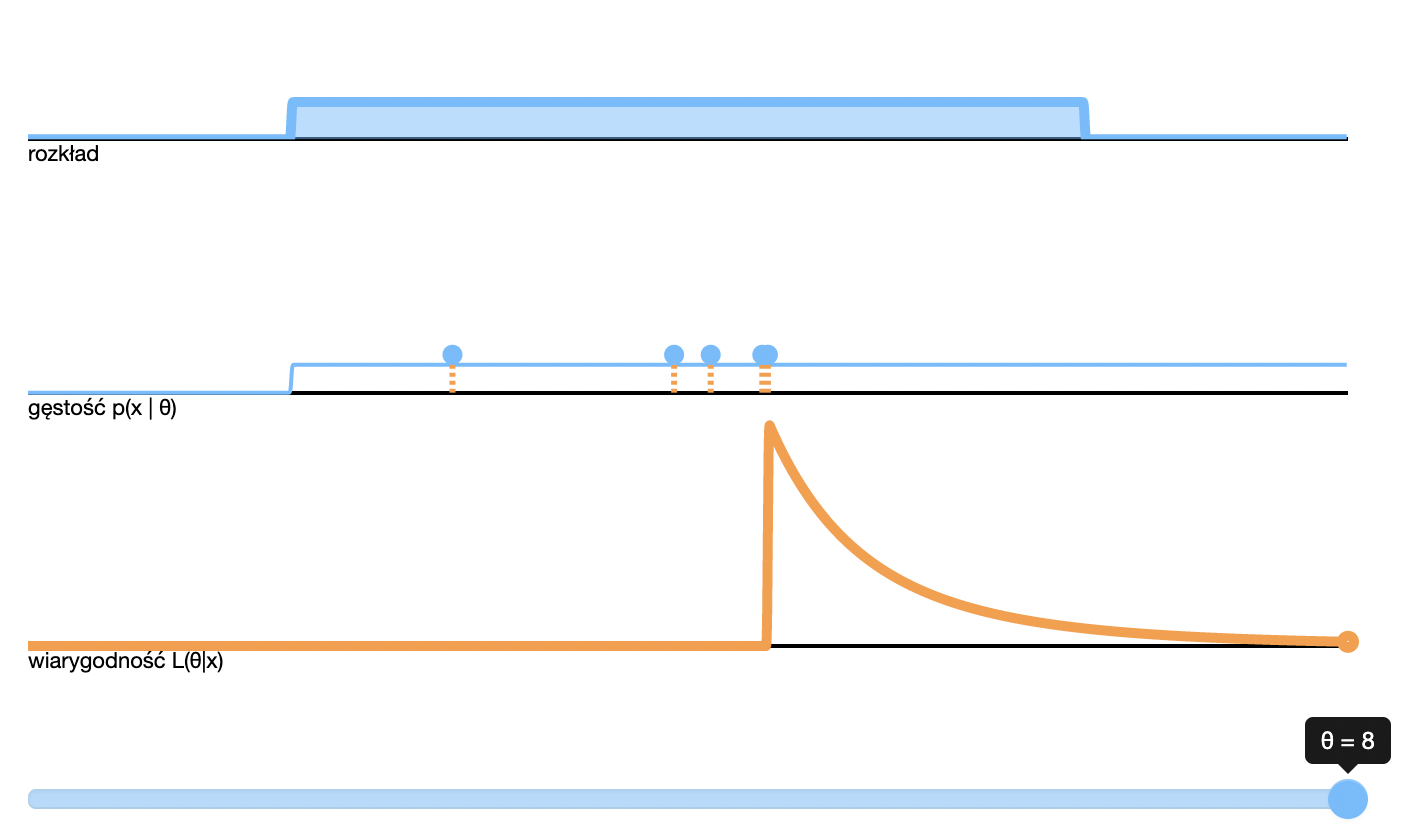
\includegraphics[scale=0.27]{images/likelihood-uniform}
        \caption{Rozkład jednostajny $(0, \theta)$ (rozmiar próbki - 5).}
    \end{minipage}
    \begin{minipage}{0.45\textwidth}
        \centering
        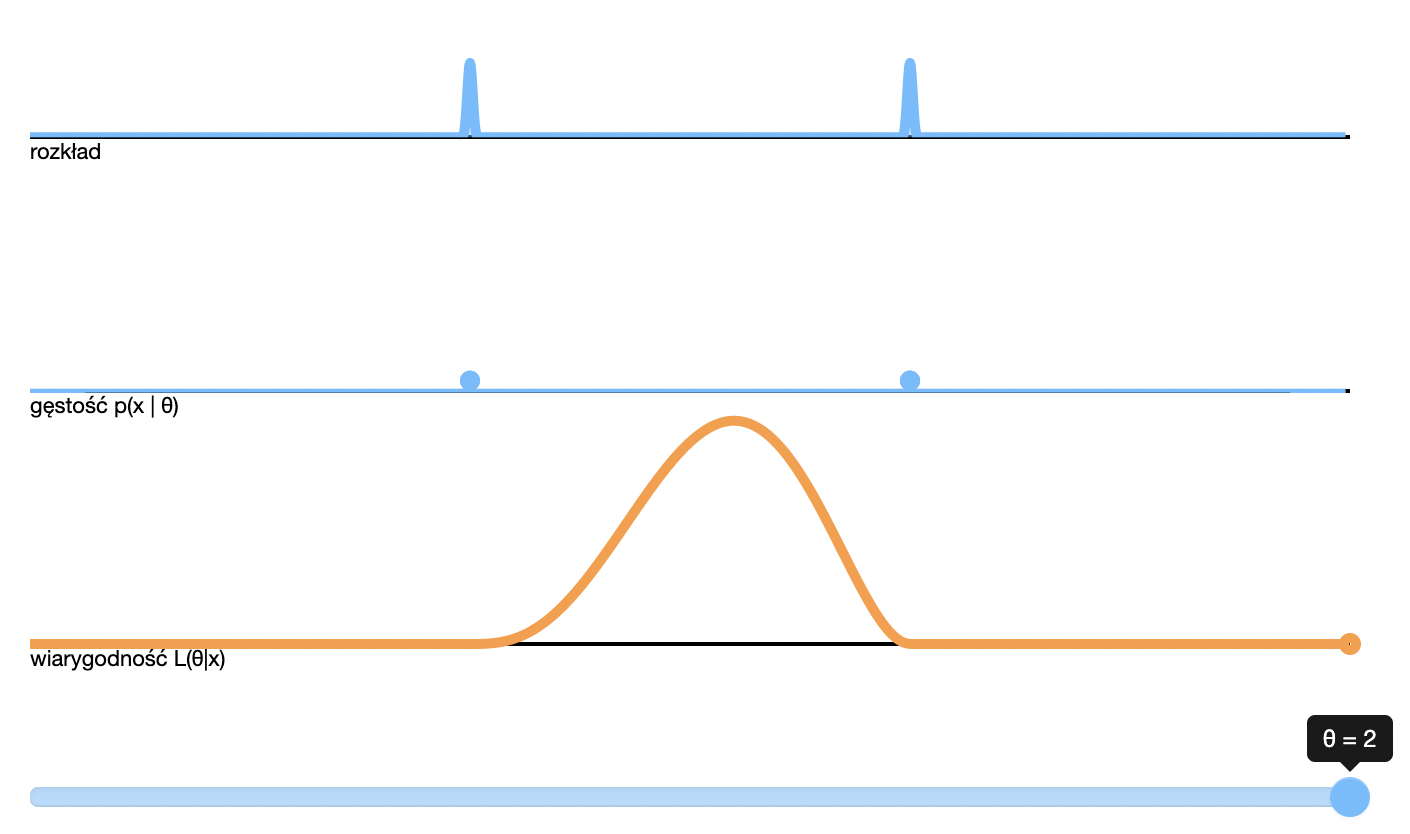
\includegraphics[scale=0.27]{images/likelihood-zero-one}
        \caption{Rozkład zero jedynkowy $(0, \theta)$ (rozmiar próbki - 5).}
    \end{minipage}
\end{figure}

\begin{align*}
    \text{Twierdzenie Bayesa: } & & P(A|B)=\frac{P(B|A) P(A)}{P(B)} \\
    \text{Funkcja wiarygodności: } & & L(\theta|x)=P(x|\theta) \\
    \text{Iloraz wiarygodności: } & & \Lambda(\theta_1 : \theta_2 | x)=\frac{L(\theta_1 | x)}{L(\theta_2 | x)}
\end{align*}

W statystyce bayesowskiej \textbf{zasada niezmienniczości ilorazu funkcji wiarygodności} nie zachodzi.
Przekształcenia (tranformacja) parametru zmienia iloraz.

    \chapter{TH}
    \section{Efektywne programowanie w języku Python - Programowanie funkcyjne w Pythonie 3. Przykłady, zalety, porównanie szybkości, zarzuty odnośnie metody reduce.}
    \section{Kody i kaflowania - Kody Hamminga: konstrukcja; własności korygujące.}

\textbf{Odległość Hamminga} - wprowadzona przez Richarda Hamminga miara odmienności dwóch ciągów o takiej samej długości,
wyrażająca liczbę miejsc (pozycji), na których te dwa ciągi się różnią.
Innymi słowy jest to najmniejsza liczba zmian (operacji zastępowania elementu innym),
jakie pozwalają przeprowadzić jeden ciąg na drugi.

Przykłady:
\begin{itemize}
    \item odległość pomiędzy ciągami 10011101 i 10\textbf{1}11\textbf{0}01 wynosi 2,
    \item odległość pomiędzy ciągami zagrabić i za\textbf{t}r\textbf{ą}bi\textbf{ł} wynosi 3.
\end{itemize}

\textbf{Kod Hamminga} - liniowy kod korekcyjny.
Kod Hamminga wykrywa i koryguje błędy polegające na przekłamaniu jednego bitu (single-error correction).
Kod ten może wykrywać (ale już nie korygować) błędy podwójne (dwa jednocześnie przekłamane bity - double-error detection).
Jest to możliwe, gdy wykorzystany zostanie dodatkowy bit parzystości.

Dla porównania: prosty kod z kontrolą parzystości nie może korygować żadnych błędów
ani też nie może być używany do detekcji błędu na więcej niż jednym bicie.

\begin{tabular}{ |c|c|c|c|c|c|c|c|c|c|c| }
    \hline
    Pozycja bitu                    & 1     & 2     & 3     & 4     & 5     & 6     & 7     \\
    \hline

    Bit parzystości (p), danych (d) & $p_1$ & $p_2$ & $d_1$ & $p_4$ & $d_2$ & $d_3$ & $d_4$ \\
    \hline

    p1                              & ×     &       & ×     &       & ×     &       & ×     \\
    p2                              &       & ×     & ×     &       &       & ×     & ×     \\
    p4                              &       &       &       & ×     & ×     & ×     & ×     \\
    \hline
\end{tabular}\\

W roku 1950 Hamming przedstawił kod $(7,4)$, który kodował 4 pozycje informacyjne jako słowo 7-bitowe,
dodając 3 bity parzystości.
Macierz generująca $G$ kodu $(7,4)$ i jego macierz kontroli parzystości $H$ są przedstawione poniżej:


\begin{align*}
    G^{T} \coloneqq \begin{pmatrix}
                        1 & 1 & 0 & 1 \\
                        1 & 0 & 1 & 1 \\
                        1 & 0 & 0 & 0 \\
                        0 & 1 & 1 & 1 \\
                        0 & 1 & 0 & 0 \\
                        0 & 0 & 1 & 0 \\
                        0 & 0 & 0 & 1
    \end{pmatrix} & &
    H \coloneqq \begin{pmatrix}
                    1 & 0 & 1 & 0 & 1 & 0 & 1 \\
                    0 & 1 & 1 & 0 & 0 & 1 & 1 \\
                    0 & 0 & 0 & 1 & 1 & 1 & 1
    \end{pmatrix}
\end{align*}

\subsection{Przykład}
Chcemy przetransmitować $1011$.
\begin{align*}
    p=\begin{pmatrix}
          d_1 \\
          d_2 \\
          d_3 \\
          d_4
    \end{pmatrix} = \begin{pmatrix}
                        1 \\
                        0 \\
                        1 \\
                        1
    \end{pmatrix}
\end{align*}
\begin{align*}
    x=G^{T}p=\begin{pmatrix}
                 1 & 1 & 0 & 1 \\
                 1 & 0 & 1 & 1 \\
                 1 & 0 & 0 & 0 \\
                 0 & 1 & 1 & 1 \\
                 0 & 1 & 0 & 0 \\
                 0 & 0 & 1 & 0 \\
                 0 & 0 & 0 & 1
    \end{pmatrix}
    \begin{pmatrix}
        1 \\
        0 \\
        1 \\
        1
    \end{pmatrix}=
    \begin{pmatrix}
        2 \\
        3 \\
        1 \\
        2 \\
        0 \\
        1 \\
        1
    \end{pmatrix}=
    \begin{pmatrix}
        0 \\
        1 \\
        1 \\
        0 \\
        0 \\
        1 \\
        1
    \end{pmatrix}
\end{align*}

Zatem $0110011$ jest kodem Hamminga odpowiadającym wiadomości $1011$.

Sprawdzamy parzystość.
\begin{align*}
    z=Hr=\begin{pmatrix}
             1 & 0 & 1 & 0 & 1 & 0 & 1 \\
             0 & 1 & 1 & 0 & 0 & 1 & 1 \\
             0 & 0 & 0 & 1 & 1 & 1 & 1
    \end{pmatrix}
    \begin{pmatrix}
        0 \\
        1 \\
        1 \\
        0 \\
        0 \\
        1 \\
        1
    \end{pmatrix}=
    \begin{pmatrix}
        2 \\
        4 \\
        2
    \end{pmatrix}=
    \begin{pmatrix}
        0 \\
        0 \\
        0
    \end{pmatrix}
\end{align*}
Wynikiem jest wektor zerowy - odbiorca może stwierdzić, że nie doszło do przekłamania.

W przeciwnym wypadku występuje korekcja błędu.
\[
    r = x + e_i
\]
gdzie $e_i$ to wektor zerowy z jedynką na pozycji $i$.
\[
    Hr=H(x+e_i)=Hx+He_i
\]
Zauważmy, że x to oryginalna wiadomość, stąd $Hx=\mathbf{0}$.
\[
    r=x+e_5=
    \begin{pmatrix}
        0 \\
        1 \\
        1 \\
        0 \\
        0 \\
        1 \\
        1
    \end{pmatrix}+
    \begin{pmatrix}
        0 \\
        0 \\
        0 \\
        0 \\
        1 \\
        0 \\
        0
    \end{pmatrix}=
    \begin{pmatrix}
        0 \\
        1 \\
        1 \\
        0 \\
        1 \\
        1 \\
        1
    \end{pmatrix}
\]
\begin{align*}
    z=Hr=\begin{pmatrix}
             1 & 0 & 1 & 0 & 1 & 0 & 1 \\
             0 & 1 & 1 & 0 & 0 & 1 & 1 \\
             0 & 0 & 0 & 1 & 1 & 1 & 1
    \end{pmatrix}
    \begin{pmatrix}
        0 \\
        1 \\
        1 \\
        0 \\
        1 \\
        1 \\
        1
    \end{pmatrix}=
    \begin{pmatrix}
        3 \\
        4 \\
        3
    \end{pmatrix}=
    \begin{pmatrix}
        1 \\
        0 \\
        1
    \end{pmatrix}
\end{align*}
\textbf{Syndrom} $101$ odpowiada wartości 5 - stąd wnioskujemy, że piąty bit jest przekłamany.
\[
    r_{corrected}=\begin{pmatrix}
                      0       \\
                      1       \\
                      1       \\
                      0       \\
                      \bar{1} \\
                      1       \\
                      1
    \end{pmatrix}=\begin{pmatrix}
                      0 \\
                      1 \\
                      1 \\
                      0 \\
                      0 \\
                      1 \\
                      1
    \end{pmatrix}
\]
Dekodowanie. Najpierw, definiujemy macierz $R$.
\begin{align*}
    R=&\begin{pmatrix}
           0 & 0 & 1 & 0 & 0 & 0 & 0 \\
           1 & 0 & 0 & 0 & 1 & 0 & 0 \\
           1 & 0 & 0 & 0 & 0 & 1 & 0 \\
           0 & 0 & 0 & 0 & 0 & 0 & 1
    \end{pmatrix}
\end{align*}
Dalej obliczamy otrzymaną wartość.
\begin{align*}
    p_r=&Rr=\begin{pmatrix}
                0 & 0 & 1 & 0 & 0 & 0 & 0 \\
                1 & 0 & 0 & 0 & 1 & 0 & 0 \\
                1 & 0 & 0 & 0 & 0 & 1 & 0 \\
                0 & 0 & 0 & 0 & 0 & 0 & 1
    \end{pmatrix}
    \begin{pmatrix}
        0 \\
        1 \\
        1 \\
        0 \\
        0 \\
        1 \\
        1
    \end{pmatrix}=
    \begin{pmatrix}
        1 \\
        0 \\
        1 \\
        1
    \end{pmatrix}
\end{align*}

    \section{Modelowanie systemów liczących - Graf sieci Petriego i jego zastosowanie w modelowaniu systemów liczących. Podaj przykłady możliwych zastosowań sieci Petriego. }
    \section{Obliczalność i złożoność - Problemy rozstrzygalne, częściowo rozstrzygalne i nierozstrzygalne; podać przykład problemów z każdej z tych klas. Podać dowód nierozstrzygalności przykładowego problemu. }

    \section{Statystyka bayesowska - Podaj twierdzenie Bayesa. Czym różni się wnioskowanie bayesowskie od wnioskowania częstotliwościowego stosowanego w podejściu klasycznym? }
    \section{Zarządzanie projektami IT - Inżynieria wymagań w projekcie: wymień przykładowe metody pozyskiwania, dokumentowania, walidacji i zarządzania wymaganiami. }



\end{document}